% !TEX root = ../../Main.tex
\fancychapter{Implementation}
\label{Chapter:Implementation}

\Cref{Chapter:RelatedWork} showed what the reviewed literature leaves open. This chapter describes what was built to address it. It covers the environment the agent trades in, the agent itself, and the procedure used to train the agent and to choose one model for each currency pair.

The sections follow this order on purpose. The agent cannot be described without its environment, because the environment gives the agent its observations and charges it for its actions. No number the agent produces means anything unless that environment is accurate. So the framework comes first, then the agent, and then the experimental procedure.

% !TEX root = ../../Main.tex
\section{Trading Framework: The Environment the Agent Trades In}
\label{Section:TradingFramework}

No existing framework could both train an agent offline on quote-level history and run the same agent on a live account without rewriting it. Building one took a large part of the effort in this work. Its design choices decide how far the results in \Cref{Chapter:ExperimentalResults} can be trusted. Three properties were required. First, the tested system and the deployed system had to be the same code, so that a result obtained offline says something about live behaviour. Second, the data had to have a fine enough resolution to rebuild the price path inside a bar, because that path decides what a position actually paid. Third, the costs had to be the costs of a real account, not simplified values chosen for convenience.

\subsection{System Architecture: Three Execution Contexts}

The framework has to be written in two languages. The strategy logic, the learning models and the market abstractions are written in Python, which has the numerical and machine learning libraries. Access to the broker is written in C\#, because cTrader \cite{noauthor_forex_nodate} runs algorithmic strategies as cBots on the .NET runtime and offers no other way to reach its order book. The two parts communicate through named memory-mapped files with paired auto-reset event handles, one pair for each direction. They work as a single-slot request and response exchange. The platform writes an update and signals. Python reads it, writes an action and signals back, and then the platform continues. Two kinds of message cross this boundary. Updates go from the platform to Python, and actions go the other way. \Cref{Figure:SystemArchitecture} shows the arrangement. The important result of this design is that the strategy object does not know where its updates come from. The same class, with the same weights, runs in three contexts.

\begin{figure}[htb!]
\centering
\begin{tikzpicture}[
  node distance=6mm,
  box/.style={draw, rounded corners=2pt, align=center, font=\small, minimum height=8mm, inner sep=3pt},
  wide/.style={box, text width=34mm},
  narrow/.style={box, text width=26mm},
  lbl/.style={font=\scriptsize\itshape},
  flow/.style={-stealth, thick},
  dashflow/.style={-stealth, thick, dashed}
]
\node[wide] (broker) {Broker\\\scriptsize IC Markets, raw spread, swap-free};
\node[wide, below=of broker] (platform) {cTrader platform};
\node[wide, below=of platform] (cbot) {Connector cBot\\\scriptsize C\# / .NET};
\node[narrow, right=14mm of cbot] (bridge) {Shared memory\\\scriptsize updates $\rightarrow$\\\scriptsize $\leftarrow$ actions};
\node[wide, right=14mm of bridge] (library) {Python library};
\node[narrow, above=8mm of library] (market) {Market abstractions\\\scriptsize ticks, bars, indicators};
\node[narrow, above=8mm of market] (strategy) {Strategy\\\scriptsize DDPG agent};
\node[narrow, below=8mm of library] (portfolio) {Portfolio\\\scriptsize orders, positions, costs};
\node[wide, below=14mm of cbot] (database) {Market database\\\scriptsize PostgreSQL, quote level};

\draw[flow] (broker) -- (platform);
\draw[flow] (platform) -- (cbot);
\draw[flow] (cbot) -- (bridge);
\draw[flow] (bridge) -- (library);
\draw[flow] (library) -- (market);
\draw[flow] (market) -- (strategy);
\draw[flow] (library) -- (portfolio);
\draw[flow] (platform.east) to[out=0, in=90] (bridge.north);
\draw[dashflow] (database) -| (library);
\node[lbl, below=1mm of database] {offline replay bypasses the platform};
\end{tikzpicture}
\caption{Framework architecture. The strategy receives updates and returns actions. It does not know whether the updates come from a live account, from the platform's own backtester or from the stored quote database.}
\label{Figure:SystemArchitecture}
\end{figure}

In the first context the platform is not used. Python replays stored quotes directly from the market database. This is the fastest of the three contexts, and it is the one used for training and for every result reported in this work. In the second context the strategy runs inside cTrader's own backtesting tab on the platform's historical data. This gives an independent check of the offline engine. In the third context the same strategy runs on a live account. It receives real quotes and sends real orders. The benefit of this design is that the three contexts differ only in where the updates come from. When a strategy behaves one way in a backtest and another way when deployed, the usual cause is two separate implementations that have diverged over time. Here there is only one implementation, so this problem does not occur.

\subsection{Market Data: Collection, Storage and Resolution}

The historical data was collected through the same connector. The C\# component requested it from cTrader, and the Python component wrote it to a local PostgreSQL database. Two types of record are stored. A tick holds the bid and ask quoted at one instant, together with the conversion rates needed to express a profit or loss in the account currency at that instant. A bar holds its open, high, low and close as references to the ticks that produced them. A bar is therefore a view of the tick tape, not a separate copy of the prices. \Cref{Tables:DataInventory} lists the data held for the seven pairs. The tick tape is the primary record, and the bar series are derived from it. This is what allows the engine to rebuild the path a price took inside a bar, instead of interpolating between its end points.

% !TEX root = ../Main.tex
\begin{table}[htb!]
\centering
\footnotesize
\caption{Market data collected from cTrader and stored locally, from January 2014 to August 2026. The tick tape takes 295 GB and is the primary record. The bar series point to the ticks that produced them.}
\label{Tables:DataInventory}
\begin{tabular}{@{}lrrrrr@{}}
\toprule
\textbf{Pair} & \textbf{Ticks} & \textbf{M1 bars} & \textbf{H1 bars} & \textbf{D1 bars} & \textbf{MN1 bars} \\
\midrule
AUD/USD & 227,914,614 & 4,643,990 & 78,320 & 3,346 & 150 \\
EUR/USD & 242,847,954 & 4,636,138 & 78,145 & 3,339 & 150 \\
GBP/USD & 281,490,557 & 4,648,216 & 78,311 & 3,339 & 150 \\
NZD/USD & 203,788,307 & 4,631,614 & 78,282 & 3,339 & 150 \\
USD/CAD & 228,356,007 & 4,635,179 & 78,319 & 3,347 & 150 \\
USD/CHF & 194,186,979 & 4,621,503 & 78,307 & 3,338 & 150 \\
USD/JPY & 284,430,458 & 4,638,775 & 78,151 & 3,338 & 150 \\
\midrule
\textbf{Total} & \textbf{1,663,014,876} & \textbf{32,455,415} & \textbf{547,835} & \textbf{23,386} & \textbf{1,050} \\
\bottomrule
\end{tabular}
\end{table}

Two properties of this data must be stated, because otherwise both would look like defects.

Bars are stamped at the close of the broker's trading session, not at midnight. This is at 22:00 UTC, or at 21:00 under daylight saving. A daily series therefore has five bars in a normal week, stamped Sunday to Thursday, and the bar stamped Thursday holds Friday's session. An audit against a calendar-day reference reports every Friday as missing. This is a result of the stamping convention, and no data is lost. The period from 11 to 25 January 2016 is missing from all seven pairs, both in ticks and in bars. The gap comes from the broker. A new download of those days returned nothing, which confirmed that the gap cannot be repaired. The gap is the same for all seven pairs, so it does not bias any comparison between them. It also falls outside the evaluation window used in \Cref{Chapter:ExperimentalResults}.

\subsection{Cost Model: Spread, Commission and Account Type}

The execution engine advances on ticks, not on bar closes. A position opened during a bar is filled at a quote that existed within that bar. A stop or target attached to it is tested against the quotes in the order they arrived. This matters for the reason given in \Cref{Chapter:RelatedWork}. A bar reports four prices but hides the order in which the price reached them. That order decides whether a stop was reached before a target, and which spread was crossed.

The account modelled is a swap-free raw-spread retail account. Each of the three charges described in \Cref{Section:PerformanceMeasurement} is applied at the rate that such an account pays. A buy is filled at the ask and a sell at the bid, both read from the tick tape at the instant of the fill. The spread is therefore charged by construction, as part of every fill, and is not deducted afterwards. The commission is charged on traded volume at $3.5$ points per side. For a standard lot of $100{,}000$ units this is $3.5$ units of the quote currency per side, or $7$ per round turn. The swap is zero. On a swap-free account this is the rate the account really charges, so it is not an approximation. \Cref{Tables:CostModel} lists the full configuration.

% !TEX root = ../Main.tex
\begin{table}[htb!]
\centering
\footnotesize
\caption{Cost and account configuration applied to every evaluation reported in this work.}
\label{Tables:CostModel}
\begin{tabularx}{\textwidth}{@{}llX@{}}
\toprule
\textbf{Setting} & \textbf{Value} & \textbf{Meaning} \\
\midrule
Account type & Raw spread, swap-free & An account that a retail client can open, with the interbank spread and no charge for overnight financing \\
\addlinespace
Spread & Accurate & The bid-ask difference recorded at the moment of the trade, read from the tick tape and not assumed \\
\addlinespace
Commission & 3.5 points per side & Charged on traded volume. This is 3.5 units of the quote currency per standard lot per side, or 7 per round turn \\
\addlinespace
Swap & 0 points & The rate a swap-free account charges, so not an approximation \\
\addlinespace
Account currency & EUR & Profit and loss converted at the rate recorded on the tick that produced it \\
\addlinespace
Initial balance & 10,000 & Reported across five starting balances, as described in \Cref{Chapter:ExperimentalResults} \\
\addlinespace
Leverage & 30 & The retail limit for major currency pairs \\
\addlinespace
Position mode & Netting & One net position per instrument, not separate hedged positions \\
\bottomrule
\end{tabularx}
\end{table}

The choice to read the spread from the ticks, instead of assuming a value for it, should be supported with data. Assuming a value is common, and the error it causes is not small. \Cref{Figure:SpreadOverTime} plots the monthly mean spread of each pair across the evaluation window. For EUR/USD, the most liquid pair in the market, the monthly mean goes from $0.77$ to $13.00$ points. This is a factor of seventeen between the quietest month and the busiest one. USD/CHF reaches $37.82$ points in January 2015, when the Swiss National Bank removed its floor against the Euro. For each of the seven pairs, the spread in the widest month is at least five times the spread in the narrowest month.

\begin{figure}[htb!]
\centering
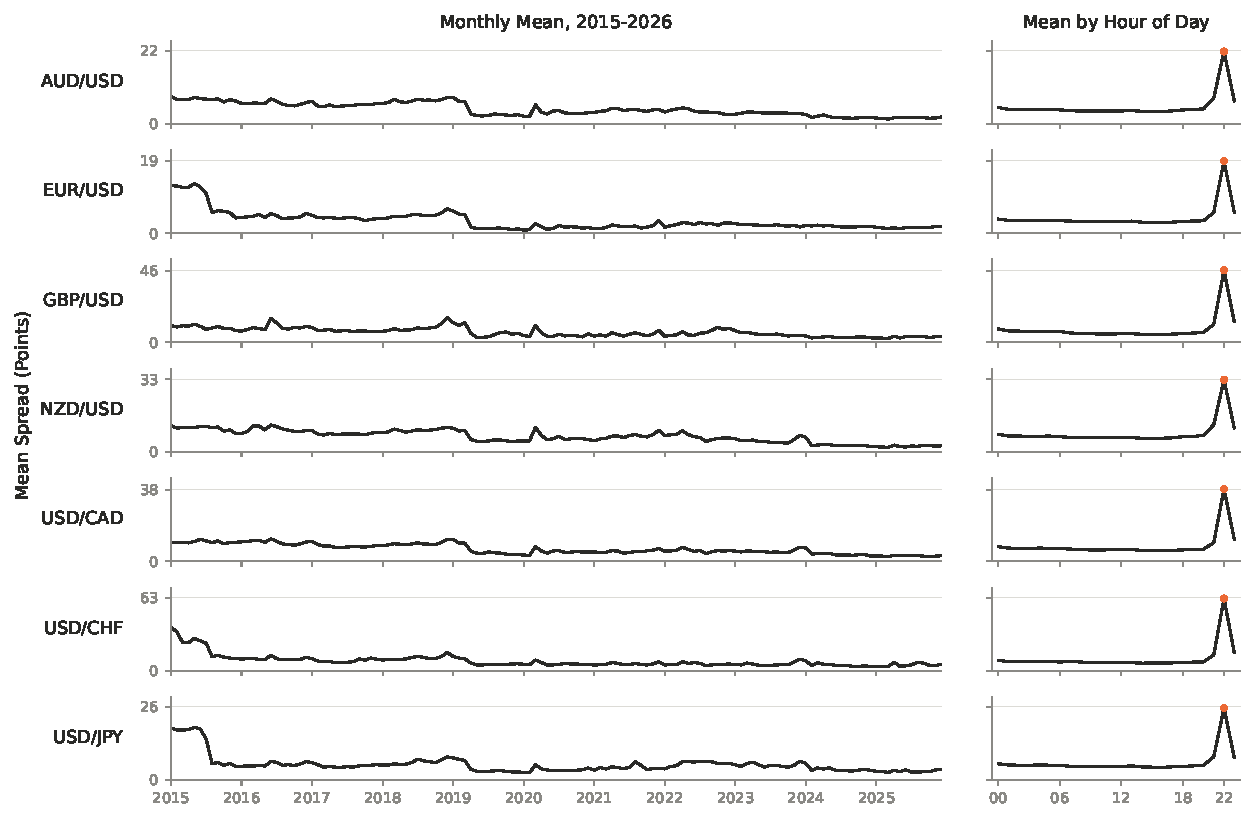
\includegraphics[width=\textwidth]{Images/SpreadOverTime.pdf}
\caption{Monthly mean spread in points for the seven major pairs, 2015 to 2026, computed from the full tick tape. EUR/USD is drawn in black. A model evaluated at a fixed spread is evaluated in market conditions that do not occur in any month of this sample.}
\label{Figure:SpreadOverTime}
\end{figure}

The pattern of this variation matters more than its size. Spreads widen when liquidity falls and around the events that move prices. These are the moments when a model trained on an average spread is most likely to act. A strategy charged a constant spread is therefore charged the wrong amount, and the error is correlated with its own trading activity. The error also goes in the direction that makes the strategy look better.

The engine was validated against cTrader's own backtester, not against itself. Six reference configurations were used, covering two currency pairs and three windows. In all of them, the engine's trade, position, order and deal records reproduce the platform's output byte for byte. The conversion of profit and loss into the account currency was also checked separately against the platform's own figures. The only divergence is sub-pip. It comes from the resolution of the stored quotes, not from the accounting. The engine therefore reproduces the platform it was built against, and it can also do more than that platform. The same strategy is evaluated offline directly on the tick tape. This runs at a speed that the platform's own backtester cannot reach, and over windows that the backtester will not cover. The cost model can be set to any account the broker offers, not only to the account the terminal happens to be connected to.

Two consequences follow. Both are stated here so that \Cref{Chapter:ExperimentalResults} can be read correctly. First, the returns reported in this work are net of the spread actually quoted and of a real commission schedule. They are therefore lower than the same policy would show on bar closes with a fixed spread or no spread, and they cannot be compared directly with results obtained in that way. Second, because the account is swap-free, no financing cost is estimated or left out. A strategy that holds positions over many nights is charged exactly what such an account would charge it.

% !TEX root = ../../Main.tex
\section{Agent Design: Observation, Action and Reward}
\label{Section:AgentDesign}

The environment of \Cref{Section:TradingFramework} supplies prices and charges for trades. Three more decisions are needed to turn it into a reinforcement learning problem: what the agent sees, what it is allowed to do, and what it is rewarded for. This section states these three decisions and then describes the algorithm that learns from them. Each decision is given with the reason for it. In every case the alternative was tried and worked worse, and those failures are part of the result.

\subsection{Observation Space: Indicators, Encoding and Normalisation}

The agent observes a vector of $38$ values at each hourly bar. None of these values is a raw price. A price level carries no information that the agent can generalise from. A policy learned at a price of $1.05$ has no reason to work at $1.20$, and in eleven years of history the price moves by more than that. Every feature is therefore a ratio, and the whole observation is dimensionless. Sixteen technical indicators, listed in \Cref{Tables:Observation}, give the market context. They are split into a fast group, which describes the last hours to days, and a slow group, which describes regimes that last months. This lets the agent tell a move within a trend apart from a change of trend.

% !TEX root = ../Main.tex
\begin{table}[htb!]
\centering
\footnotesize
\caption{The sixteen technical indicators forming the market context of the observation. Periods are in hourly bars. Each moving average contributes two features, its distance from price and its own differential, both in units of the average true range; each momentum reading contributes one, scaled by the movement expected over its lookback.}
\label{Tables:Observation}
\begin{tabularx}{\textwidth}{@{}llrX@{}}
\toprule
\textbf{Indicator} & \textbf{Family} & \textbf{Period} & \textbf{Role in the observation} \\
\midrule
ATR & Volatility & 14 & Volatility unit; divides every trend feature and sets the stop distance \\
\addlinespace
RV (fast) & Volatility & 16 & Short-horizon realised volatility; divides the momentum features \\
RV (slow) & Volatility & 480 & Long-horizon realised volatility; its ratio to the fast reading gives the volatility regime \\
\addlinespace
ER & Trend & 120 & Efficiency ratio; how directional recent movement has been, bounded in $[0, 1]$ \\
\addlinespace
ROC Fast & Momentum & 24 & One day \\
ROC Medium & Momentum & 120 & One week \\
ROC Slow & Momentum & 480 & One month \\
ROC Regime & Momentum & 1{,}440 & One quarter \\
ROC Epoch & Momentum & 2{,}880 & Two quarters \\
\addlinespace
SMA Fast & Trend & 24 & One day \\
SMA Medium & Trend & 120 & One week \\
SMA Slow & Trend & 480 & One month \\
SMA Regime & Trend & 1{,}440 & One quarter \\
SMA Epoch & Trend & 2{,}880 & Two quarters \\
SMA Cycle & Trend & 4{,}320 & Three quarters \\
SMA Era & Trend & 5{,}040 & Roughly one year \\
\bottomrule
\end{tabularx}
\end{table}

The indicator values are encoded as follows. Here $C$ is the bar close, $\sigma_f$ and $\sigma_s$ are the fast and slow realised volatilities, $A$ is the average true range, and $M_i$ is the $i$-th moving average, with period $N_i$:

\begin{equation}
\frac{A}{C}, \qquad \sigma_f, \qquad \ln\!\left(\frac{\sigma_f}{\sigma_s}\right), \qquad \text{ER}
\label{Equation:VolatilityFeatures}
\end{equation}

\begin{equation}
\frac{\text{ROC}(N_j)}{\sigma_f \sqrt{N_j}}, \qquad \frac{C - M_i}{A}, \qquad \frac{M_i - M_i^{-1}}{A}
\label{Equation:TrendFeatures}
\end{equation}

Each formula removes a different dependence. Dividing the average true range by the close gives volatility as a fraction of the price. The logarithm of the ratio of fast to slow volatility shows the volatility regime. It is zero when the two agree, positive when volatility is rising and negative when it is falling. Dividing a momentum reading by $\sigma_f \sqrt{N_j}$ scales it by the movement expected over that lookback under a random walk. A value near one then means a move of normal size, whatever the period. The distance from a moving average, measured in units of the average true range, says how far the price is from its trend compared with the current volatility. The differential of the same quantity gives the direction in which the trend is moving. The other features are the position in the calendar, encoded as four sine and cosine pairs, the current signed exposure as a fraction of the largest position the account could hold, and six values that describe the last bar as log returns of its open, high, low and close against the previous close, divided by $\sigma_f$.

Features that are not bounded by construction are standardised with a causal exponentially weighted z-score, with $\alpha = 1/200$. Here $x_t$ is a raw value, and $\mu_t$ and $s^2_t$ are its running mean and variance:

\begin{equation}
z_t = \frac{x_t - \mu_{t-1}}{\sqrt{s^2_{t-1} + \epsilon}}
\label{Equation:Normalisation}
\end{equation}

\begin{equation}
\mu_t = \mu_{t-1} + \alpha \delta_t, \qquad s^2_t = (1 - \alpha)\left(s^2_{t-1} + \alpha \delta_t^2\right), \qquad \delta_t = x_t - \mu_{t-1}
\label{Equation:NormalisationUpdate}
\end{equation}

The subscript $t-1$ in \Cref{Equation:Normalisation} is the most important detail of this design. A value is standardised with statistics that end at the previous step. Only after that is the value added to those statistics. A z-score computed over the whole sample would leak future information into every observation, and it would inflate every result derived from it. Features that are already bounded, such as the exposure fraction, the efficiency ratio and the calendar encodings, have a flag that skips this layer, so their natural range is kept.

\subsection{Action Space: Position Sizing and Risk}

The agent outputs a single continuous value $a \in [-1, 1]$. Its sign is the direction of the position, and its magnitude is the fraction of a reference size to hold. Direction and size are therefore set by one decision. The discrete action sets reviewed in \Cref{Chapter:RelatedWork} cannot express this. The reference size is fixed-fractional. Let $B$ be the account balance, $\rho$ the risk fraction per position, and $k$ the stop distance in multiples of the average true range. The reference volume $V_{ref}$ is the volume that loses $\rho B$ if the price moves $k \cdot A$ against it. The target volume is this reference scaled by the action:

\begin{equation}
V_{target} = a \cdot V_{ref}, \qquad V_{ref} = \frac{\rho \, B}{k \, A}
\label{Equation:PositionSizing}
\end{equation}

with $\rho = 1\%$ and $k = 1.5$ throughout this work. The agent therefore never chooses an absolute number of units. It chooses a fraction of a size that the risk rule has already set, and this size becomes smaller on its own as volatility rises.

One defect in this calculation was found during the campaign. It is reported here because it affects one of the seven results. The volume calculation leaves out the conversion between the quote currency and the account currency. The risk actually taken is therefore $\rho / p$ and not $\rho$, where $p$ is the price of the pair. For pairs quoted close to one the difference does not matter, and the six pairs quoted against the US Dollar all take about the intended $1\%$. USD/JPY was quoted near $120$ at the start of the sample, so its effective risk is $0.008\%$. This is so small that the computed volume falls below the broker's minimum, and no position can open at all. To correct for this, $\rho$ was scaled by the price. This restores the intended risk per position and does not add leverage. \Cref{Chapter:ExperimentalResults} reports the level used for each pair. The defect is a limitation of the framework, not of the method, and it is listed as future work.

\subsection{Reward Function: Log Return, Scaling and Clipping}

The reward at each step is the log return of account equity, scaled and then clipped:

\begin{equation}
r_t = \operatorname{clip}\!\left(\lambda \ln\!\frac{E_t}{E_{t-1}},\; -c,\; +c\right), \qquad \lambda = 1000, \quad c = 1
\label{Equation:Reward}
\end{equation}

The log return is a natural choice for a trading objective because it is additive over time. The per-step rewards telescope to $\ln(E_T / E_0)$, so maximising their sum maximises the final compounded wealth. The log return also does not depend on the account size. The scale factor is needed, and the reason for it comes from a measured result. Moody and Saffell describe differential risk-adjusted rewards, which accumulate an online estimate of a Sharpe or Sortino ratio. These rewards are scale-invariant: doubling every position leaves the ratio the same. An agent that optimises such a reward gets no gradient that pushes its position size up. In this environment the policy collapses to positions of about $3\%$ of the size available to it. The resulting policy is directionally sensible, but it has no financial value. A scale-sensitive reward is therefore needed. The factor $\lambda$ raises an hourly equity log return, which is usually of order $10^{-4}$, to a magnitude that the critic can distinguish from its own approximation error.

The clip is a numerical safeguard of the kind introduced with the Deep Q-Network \cite{mnih_human-level_2015}. It is applied after the encoding. Its effect must be stated clearly here, because $\lambda$ and $c$ are not independent. Together they clip the raw log return at $\pm c / \lambda = \pm 0.1\%$. On the delivered EUR/USD model the bound is reached on $38.2\%$ of the $68\,155$ hourly steps, and the median absolute scaled reward is $0.70$. So for about two steps in five the agent is told the direction of the equity move but not its magnitude. This is a real property of the objective. It is reported here so that the learned behaviour in \Cref{Chapter:ExperimentalResults} is read against the reward the agent actually received.

\subsection{Learning Algorithm: DDPG and its Adaptations}

The algorithm is the Deep Deterministic Policy Gradient of \Cref{Section:DeepReinforcementLearning}. The actor, the critic and their delayed targets are as described there, and they are trained from a replay buffer with Ornstein-Uhlenbeck exploration noise. The equations of that section are not repeated here. The rest of this section gives the six ways in which the implementation differs from the original, each with its reason. \Cref{Tables:Hyperparameters} compares every value with the published one.

% !TEX root = ../Main.tex
\begin{table}[htb!]
\centering
\footnotesize
\caption{Hyperparameters compared with the original Deep Deterministic Policy Gradient \cite{lillicrap_continuous_2015}. Three values were changed and five mechanisms were added. The rest are the published values.}
\label{Tables:Hyperparameters}
\begin{tabularx}{\textwidth}{@{}llll X@{}}
\toprule
\textbf{Parameter} & \textbf{Original} & \textbf{This work} & \textbf{Status} & \textbf{Reason for the difference} \\
\midrule
Actor hidden layers & $400 \times 300$ & $64 \times 32$ & Changed & Noisy, non-stationary series supports less capacity \\
Discount factor $\gamma$ & $0.99$ & $0.9995$ & Changed & Horizon matched to the holding period, months and not days \\
Hidden normalisation & Batch & Layer & Changed & Inference on one observation must match training on batches \\
\addlinespace
Actor learning rate & $10^{-4}$ & $10^{-4}$ & Unchanged & \\
Critic learning rate & $10^{-3}$ & $10^{-3}$ & Unchanged & \\
Soft update rate $\tau$ & $0.001$ & $0.001$ & Unchanged & \\
Batch size $N$ & $64$ & $64$ & Unchanged & \\
Replay capacity & $10^{6}$ & $10^{6}$ & Unchanged & \\
Critic weight decay & $10^{-2}$ & $10^{-2}$ & Unchanged & \\
Noise $\theta$, $\sigma$ & $0.15$, $0.2$ & $0.15$, $0.2$ & Unchanged & \\
Final layer init & $U[-3\!\times\!10^{-3}, 3\!\times\!10^{-3}]$ & same & Unchanged & \\
\addlinespace
Gradient clip & --- & $1.0$ & Added & Bounds the size of one update caused by a rare large error \\
Warmup transitions & --- & $3{,}000$ & Added & First updates drawn from a varied buffer \\
Actor penalty $\beta$ & --- & $0.001$ & Added & Prevents saturation of the output tangent and collapse to a constant action \\
Reward scale $\lambda$ & --- & $1{,}000$ & Added & Raises an hourly log return above the critic's approximation error \\
Reward clip $c$ & --- & $1$ & Added & Numerical safeguard; limits the raw log return to $\pm 0.1\%$ \\
\bottomrule
\end{tabularx}
\end{table}

The first difference is the observation and the reward, described above.

The second is the size of the networks. The original uses hidden layers of $400$ and $300$ units for low-dimensional control tasks. Here they have $64$ and $32$ units. A $38$-dimensional observation of a noisy, non-stationary series supports much less capacity than a physics simulator with a clean reward. Larger networks fitted the training window but did not generalise beyond it. The third is the discount factor, which was raised from $0.99$ to $0.9995$. With an hourly step, $\gamma = 0.99$ gives a horizon of about a hundred bars, or about four days. This is shorter than the positions this strategy is meant to hold. At $0.9995$ the horizon grows to about two thousand bars, or roughly three months, which matches the regime indicators in the observation.

The fourth is the normalisation inside the networks. The original applies batch normalisation to the hidden layers. This implementation applies layer normalisation instead. The reason is deployment. Batch normalisation behaves differently on a single sample than on a training batch, because it depends on running statistics collected during training. On a live account, the agent must act on exactly one observation at a time. Layer normalisation normalises across the features of one sample. The computation done during training is therefore the same as the computation done in deployment. The target networks also do not need a second set of running statistics that must be kept in sync.

The fifth is gradient clipping. The original uses none. Here the gradient norm of both the actor and the critic is clipped to $1$ before each optimiser step. This limits the size of a single update. It stops a rare large temporal-difference error from moving the parameters far enough to make the critic unstable. It is only a stability measure. In particular, it does not solve the collapse discussed next, which is caused by a lack of gradient, not by too much of it.

The sixth is a penalty on the actor. This is the only change that alters the objective itself, and not just the way it is optimised. It was added because the published algorithm does not train on this problem. The actor's final layer applies a hyperbolic tangent to a pre-activation $u(s)$ to keep the action bounded. The derivative of this function vanishes as $|u|$ grows. If the policy is pushed into that region, it stops responding. The action saturates at $\pm 1$, no gradient flows back, and the agent holds one constant position for the rest of training. The fix is to penalise the magnitude of the pre-activation directly. This keeps the policy in the region where the tangent does not saturate. \Cref{Figure:ActorNetwork} shows where in the network this penalty acts:

\begin{equation}
L_{actor} = -\frac{1}{N}\sum_{i} Q\!\left(s_i, \tanh u(s_i) \,\middle|\, \theta^{Q}\right) + \frac{\beta}{N}\sum_{i} u(s_i)^2
\label{Equation:ActorRegularisation}
\end{equation}

\begin{figure}[htb!]
\centering
\resizebox{\textwidth}{!}{%
\begin{tikzpicture}[
  node distance=5mm,
  layer/.style={draw, rounded corners=1.5pt, align=center, font=\scriptsize, minimum height=9mm, inner sep=3pt, text width=20mm},
  point/.style={draw, circle, inner sep=1.5pt, font=\scriptsize},
  flow/.style={-stealth, semithick},
  pen/.style={-stealth, semithick, dashed}
]
\node[layer] (s) {observation\\$s \in \mathbb{R}^{38}$};
\node[layer, right=of s] (h1) {Linear 64\\LayerNorm\\ReLU};
\node[layer, right=of h1] (h2) {Linear 32\\LayerNorm\\ReLU};
\node[layer, right=of h2] (f3) {Linear 1};
\node[point, right=6mm of f3] (u) {$u$};
\node[layer, right=6mm of u] (th) {$\tanh$};
\node[layer, right=of th] (a) {action\\$a \in [-1,1]$};
\node[font=\scriptsize, below=8mm of u, align=center] (pen) {penalty $\beta\,\overline{u^{2}}$};

\draw[flow] (s) -- (h1);
\draw[flow] (h1) -- (h2);
\draw[flow] (h2) -- (f3);
\draw[flow] (f3) -- (u);
\draw[flow] (u) -- (th);
\draw[flow] (th) -- (a);
\draw[pen] (pen) -- (u);
\end{tikzpicture}}
\caption{The actor. Layer normalisation replaces the batch normalisation of the original, so a single observation is processed exactly as a training batch is. The penalty of \Cref{Equation:ActorRegularisation} acts on the pre-activation $u$, before the tangent. This is where saturation would otherwise remove the gradient.}
\label{Figure:ActorNetwork}
\end{figure}

with $\beta = 0.001$. Setting $\beta = 0$ recovers the original actor loss exactly, so the change extends the original loss and does not replace it. Together with the scale-sensitive reward, this penalty prevents policy collapse. The two mechanisms deal with different parts of the same failure. The reward supplies a gradient that rewards larger positions, and the penalty keeps the actor in the region where that gradient can act. Everything else follows the published algorithm. The learning rates, the soft update rate, the batch size, the replay capacity, the exploration noise parameters, the critic weight decay and the layer initialisation are the values given in the original work. A warmup period of $3000$ transitions is used before learning begins. This way the first updates are drawn from a buffer with some variety in it, and not from the first few correlated steps of an episode.

% !TEX root = ../../Main.tex
\section{Experimental Procedure: Training, Selection and Deployment}
\label{Section:ExperimentalProcedure}

An agent design does not produce a result on its own. Training is stochastic, so the same configuration run twice gives two different policies. A procedure is needed to decide which of them is reported, and why. This section describes that procedure, the criteria used at each stage, and the two deployment decisions that sit between the learned policy and the orders actually sent.

\subsection{Training Procedure: Seeds, Episodes and Data Splits}

The eleven-year window is split once into three consecutive periods. The window is written as $[T_0, T_3)$, where $T_0$ is the first of January 2015 and $T_3$ is the first of January 2026:

\begin{equation}
\underbrace{[T_0, T_1)}_{\text{training, 9 years}} \quad
\underbrace{[T_1, T_2)}_{\text{validation, 1 year}} \quad
\underbrace{[T_2, T_3)}_{\text{testing, 1 year}}
\label{Equation:Split}
\end{equation}

Weights are updated on the training period only. The validation period decides which state of the network is kept. The testing period is used once, after every other decision has been made. Within this split, a single training run works as follows. A seed fixes the network initialisation, the stream of exploration noise and the order in which the replay buffer is sampled, so it determines the whole run. The agent then runs $30$ episodes. An episode is one pass over the training period. Weights are not reset between episodes. The run is a single sequence of $30$ passes, and the network at the start of episode $n+1$ is the network at the end of episode $n$. After each episode the agent is evaluated once over the validation period, with learning turned off. This evaluation is reduced to a single number, the Calmar ratio, which is the annualised return divided by the maximum drawdown. Let $f_n$ be this value and let $g_n$ be an eligibility test defined below. The state kept after episode $n$ is

\begin{equation}
\theta^{\star} \leftarrow \theta_n \quad \text{if} \quad (g_n \wedge \neg g^{\star}) \;\vee\; \left(g_n = g^{\star} \wedge f_n > f^{\star}\right)
\label{Equation:KeepBest}
\end{equation}

which prefers an eligible episode to an ineligible one, whatever the scores. Otherwise it keeps the higher score within the same eligibility class. The saved state is a copy. The run continues training from $\theta_n$, not from $\theta^{\star}$, so a later episode never restarts from an earlier checkpoint. The eligibility test $g_n$ rejects policies that are degenerate. It does not reject a policy only because it performs poorly. An episode passes only if it opened at least ten positions, spent at least three hundred bars on each side of the market, and held its weaker side for at least $30\%$ of the time it held its stronger one. A policy that never trades, or that is long for the whole period, can reach a good Calmar ratio on a trending window without having learned anything about when to hold a position. The test removes such a policy before the scores are compared. Between $128$ and $256$ seeds were run for each currency pair, and the runs differed only in the seed. \Cref{Figure:TrainingPipeline} shows how the three stages fit together.

\begin{figure}[htb!]
\centering
\begin{tikzpicture}[
  node distance=5mm,
  stage/.style={draw, rounded corners=2pt, align=center, font=\small, text width=32mm, minimum height=8mm, inner sep=3pt},
  small/.style={stage, font=\scriptsize, text width=30mm},
  note/.style={font=\scriptsize\itshape, align=left},
  flow/.style={-stealth, thick}
]
\node[stage] (seed) {Seed $s$\\\scriptsize init, noise, sampling};
\node[small, right=10mm of seed] (episode) {Episode $n$ of 30\\one pass over training};
\node[small, right=10mm of episode] (valid) {Validation pass\\learning disabled};
\node[small, below=9mm of valid] (keep) {Calmar $f_n$ + eligibility\\keep-best checkpoint};
\node[small, below=9mm of episode] (test) {Test pass\\once, after 30 episodes};
\node[stage, below=9mm of seed] (pool) {Pool of 128--256\\trained seeds};
\node[stage, below=9mm of pool] (gates) {Gates\\reject degenerate};
\node[small, right=10mm of gates] (sweep) {Risk sweep\\$\times 1.0$ to $\times 3.0$};
\node[small, right=10mm of sweep] (score) {Composite score\\percentile ranks};
\node[stage, below=9mm of gates] (champion) {Published model};

\draw[flow] (seed) -- (episode);
\draw[flow] (episode) -- (valid);
\draw[flow] (valid) -- (keep);
\draw[flow] (keep) -- node[note, above, midway] {} (test);
\draw[flow] (keep.west) to[out=180, in=0] node[note, above, midway] {\scriptsize next episode} (episode.south east);
\draw[flow] (test) -- (pool);
\draw[flow] (pool) -- (gates);
\draw[flow] (gates) -- (sweep);
\draw[flow] (sweep) -- (score);
\draw[flow] (score.south) to[out=270, in=0] (champion.east);
\end{tikzpicture}
\caption{The three stages of the procedure. The Calmar ratio chooses among the episodes of one seed. The composite score of \Cref{Section:ExperimentalProcedure} chooses among seeds.}
\label{Figure:TrainingPipeline}
\end{figure}

One property of this setup must be stated clearly, because it limits what the results in \Cref{Chapter:ExperimentalResults} can claim. The split of \Cref{Equation:Split} applies to the training of a single seed. The choice of which seed to publish, described next, is based on performance over the whole eleven-year window. The performance figures reported in this work are measured over that same window. The testing period is therefore held out from the training of each candidate and from the choice among its episodes. It is not held out from the choice among candidates, so the headline returns are not out-of-sample estimates. This is the weakest point of the method, and it is not hidden anywhere in the rest of this thesis.

\subsection{Model Selection: Gates and Composite Ranking}

Once the seeds for a pair have been trained, each one is evaluated over the full window with the cost model of \Cref{Tables:CostModel}, and one is chosen. The choice is made in two steps, first rejection and then ranking, because they answer two different questions. The first question is whether a policy is admissible at all. The second is which of the admissible policies is best.

Four gates reject a candidate directly. First, its return must be positive. Second, its weaker direction must make up at least $10\%$ of its exposure. This removes policies that are long or short the whole time. Third, its mean holding period must be at least twenty-four bars. This removes policies whose signal is noise. Fourth, its regime score must be higher than the score of the same policy with its position sequence rotated in time. The regime score is the fraction of market movement during which the policy held the correct position. The last gate needs some explanation, because a fixed threshold was tried first and does not work. A rotated policy holds the same positions for the same durations, but at the wrong moments. Its score therefore measures what the policy's autocorrelation and holding pattern would earn by luck alone. Across the seven pairs these null scores range from $48$ to $70$. A fixed threshold of, for example, $55$ would be below chance on one pair and too strict on another. The null score is therefore computed for each model and not assumed.

Candidates that pass the gates are ranked by a composite of percentile ranks within their own pool. For a metric $m$ and a pool of $K$ candidates, the rank of candidate $i$ is

\begin{equation}
R_m(i) = 100 \cdot \frac{\left|\left\{ j : v_m(j) < v_m(i) \right\}\right|}{K - 1}
\label{Equation:PercentileRank}
\end{equation}

where $v_m$ is negated for metrics that are better when smaller, such as drawdown. The metrics are split into three groups, listed in \Cref{Tables:Composite}. The score is the unweighted mean of the three group means:

\begin{equation}
S(i) = \frac{1}{3} \sum_{G \in \{\text{money}, \text{safety}, \text{behaviour}\}} \frac{1}{|G|} \sum_{m \in G} R_m(i)
\label{Equation:Composite}
\end{equation}

% !TEX root = ../Main.tex
\begin{table}[htb!]
\centering
\footnotesize
\caption{Parts of the composite selection score of \Cref{Equation:Composite}. The three groups have equal weight, so return makes up one ninth of the total and does not dominate it. The ratios are those defined in \Cref{Section:PerformanceMeasurement}.}
\label{Tables:Composite}
\begin{tabularx}{\textwidth}{@{}lX@{}}
\toprule
\textbf{Group} & \textbf{Metrics, each used as a percentile rank within the candidate pool} \\
\midrule
Money & Annualised return, Calmar ratio, Sterling ratio \\
\addlinespace
Safety & Sharpe ratio, Sortino ratio, inverse maximum drawdown, inverse downside volatility \\
\addlinespace
Behaviour & Two-sidedness (the weaker exposure side as a fraction of half), regime edge over the model's own rotation null, mean holding period, longest holding period \\
\bottomrule
\end{tabularx}
\end{table}

Two design decisions are built into \Cref{Equation:Composite}. First, ranks are relative to the pool and not absolute. No threshold can therefore exclude a candidate that is simply better than all the others in its pool. Second, the three groups have equal weight, so a policy cannot win on return alone. Money, safety and behaviour each count for a third. A candidate with the highest return in its pool, but with no two-sidedness and no regime edge over its rotation null, scores poorly on two groups out of three. Each candidate that passes the gates is also evaluated at several position sizes, from the reference risk of \Cref{Equation:PositionSizing} up to three times that risk. Scaling the risk fraction changes only the size of the positions the policy takes. It does not change the learned policy. The level chosen for each pair is reported with the results.

\subsection{Deployment: Decision Frequency and Rebalance Threshold}

Two decisions sit between the learned policy and the orders that are actually sent. Together they explain more of the delivered performance than any hyperparameter.

The first is the decision frequency, which is how often the agent may act. The agent observes every hourly bar, but it may act only once per calendar day. A key is built from the timestamp of each bar, and a new action is taken only when that key changes:

\begin{equation}
\kappa(t) = (\text{year}(t), \text{month}(t), \text{day}(t))
\label{Equation:DecisionKey}
\end{equation}

The key is built from the calendar and not from a count of bars. This means that the gaps and short sessions described in \Cref{Section:TradingFramework} do not affect it. A week with a holiday still produces one decision per trading day, and the decisions stay aligned with the trading days. The second decision is a rebalance threshold. A continuous action changes slightly at every decision. Acting on every such change would send a stream of tiny orders, and each of them would pay the spread and a commission. An order is therefore sent only when the change in the target position is large enough to be worth its cost:

\begin{equation}
\left| V_{target} - V_{current} \right| \;\geq\; \max\!\left(V_{min},\; \eta \left| V_{ref} \right|\right), \qquad \eta = 0.20
\label{Equation:Hysteresis}
\end{equation}

where $V_{min}$ is the broker's minimum volume. The threshold is a fraction of the reference volume, not of the position currently held, so it does not shrink to zero as a position is reduced. \Cref{Tables:Deployment} isolates the effect of each decision, measured on one model with nothing retrained. The comparison is between four configurations of the same weights, so the differences are attributable to the deployment layer alone.

% !TEX root = ../Main.tex
\begin{table}[htb!]
\centering
\footnotesize
\caption{Effect of the two deployment decisions, measured on one EUR/USD model over the full window with nothing retrained. All four rows use the same weights with different execution settings, so the differences are attributable to the deployment layer alone. This model comes from before the seven-pair campaign and is used here only to isolate the effect of each decision.}
\label{Tables:Deployment}
\begin{tabular}{@{}llrrrr@{}}
\toprule
\textbf{Frequency} & \textbf{Threshold} & \textbf{Commission} & \textbf{Return} & \textbf{Sharpe} & \textbf{Max drawdown} \\
\midrule
Daily & --- & none & $+42.48\%$ & $0.319$ & $24.4\%$ \\
Hourly & --- & none & $-38.57\%$ & $-0.308$ & $50.5\%$ \\
Hourly & --- & 3.5 points & $-64.70\%$ & $-0.732$ & $70.5\%$ \\
Daily & $0.20$ & 3.5 points & $+34.02\%$ & $0.275$ & $23.5\%$ \\
\bottomrule
\end{tabular}
\end{table}

Two things follow from that table. First, moving from hourly to daily decisions adds about eighty percentage points and turns a losing configuration into a profitable one. The reason is that hourly decisions act on noise that the eleven-year horizon of the discount factor was never meant to capture. Second, the rebalance threshold recovers about twelve percentage points under realistic costs, and at the same time it reduces drawdown instead of increasing it. This is unusual. Commission alone costs over twenty percentage points without the filter and about six with it. The continuous action space makes the strategy expressive, and this filter keeps its trading costs low enough.

\subsection{Worked Example: One Position From Decision to Settlement}

The earlier parts of this chapter define each component separately. This section follows one position through all of them, using a trade taken by the delivered EUR/USD model. This allows the arithmetic to be checked instead of taken on trust.

At 02:00 on 30 January 2019 the daily decision key of \Cref{Equation:DecisionKey} changed, and the agent was asked for an action for the first time that day. It received the 38-value observation of \Cref{Section:AgentDesign}, built from the bar that had just closed, and it returned a positive action. At that moment the reference volume of \Cref{Equation:PositionSizing} risked $1\%$ of the balance over a stop of $1.5$ average true ranges. The action scaled this volume, and the result was rounded to the broker's volume step. This gave a target of $12{,}000$ units of the base currency. The change from the position held at that time was larger than the threshold of \Cref{Equation:Hysteresis}, so an order was sent. The tick recorded at that instant quoted $1.14392$ ask and $1.14387$ bid, a spread of five points. The buy was filled at the ask. Twenty-four hours later the key changed again, and the agent's action changed sign. The position was closed at the bid quoted at that time, $1.14931$. The profit follows from those two prices and the volume. It is expressed in the account currency at the conversion rate recorded on the closing tick:

\begin{equation}
12{,}000 \times \left(1.14931 - 1.14392\right) = 64.68 \text{ USD} \;\;\longrightarrow\;\; 56.27 \text{ EUR}
\label{Equation:WorkedGross}
\end{equation}

The spread is already included in that figure. It was paid at entry, by filling at the ask and not at the mid, and again at exit, by filling at the bid. This is why the round trip crosses the spread exactly once. The commission is charged separately at both ends:

\begin{equation}
2 \times 3.5 \times 10^{-5} \times 12{,}000 = 0.84 \text{ USD} \;\;\longrightarrow\;\; 0.72 \text{ EUR}
\label{Equation:WorkedCommission}
\end{equation}

The position was held overnight, but the swap is zero because the account is swap-free. The position therefore settled at $56.27 - 0.72 = 55.55$ EUR, which is the figure in the exported trade record. One trade says little on its own. The delivered EUR/USD model took $1{,}777$ trades over the eleven years. Across all of them, the same accounting gives a gross profit of $8{,}733.62$ EUR, a commission charge of $1{,}669.50$ EUR and a swap charge of exactly zero, for a net of $7{,}064.12$ EUR. Commission alone took $19.1\%$ of the gross profit. This figure does not include the spread, which cannot be separated from the gross figure because it is part of every fill. A result reported without these charges would describe a different strategy.

Everything described here was fixed before any result was seen. There is one architecture, one observation, one reward and one selection rule, and they were applied unchanged to seven instruments. This is what makes the results comparable across pairs.

It also makes the results falsifiable, because they can show the design to be wrong. A design that is tuned on one instrument until it works can always be made to work on that instrument. Its results then cannot tell a real strategy apart from a description of that instrument's past prices. When the same design is applied to seven instruments, a failure on any of them shows in the results. The results in \Cref{Chapter:ExperimentalResults} include a pair on which the design does not work.